\documentclass[11pt]{article}
\usepackage{iclr2025_conference,times}
\iclrfinalcopy
% \usepackage[margin=0.6in]{geometry}
\usepackage{amsmath, amssymb}
\usepackage{graphicx}
\usepackage{booktabs}
\usepackage{hyperref}
\usepackage[compact]{titlesec}
\usepackage{enumitem}
\usepackage{indentfirst}
\usepackage{xcolor}
\usepackage{microtype}
\usepackage{float}

\usepackage{hyperref}
\usepackage{url}
\usepackage{multirow}
\usepackage{amsmath}
\usepackage{amssymb}
\usepackage{graphicx}
\usepackage{xcolor}
\usepackage{subcaption}
\usepackage{float}
\usepackage{microtype}
\usepackage{parskip}
% \usepackage[numbers]{natbib}
\usepackage{titlesec}
\usepackage{authblk}
\usepackage{tikz}

\input{math_commands.tex}
\usetikzlibrary{arrows.meta,positioning,shapes.geometric,fit,backgrounds,calc}

\title{Ask or Commit? \\ Clarification in Multimodal Reference Games\\[4pt]}

\author{Shizhe Zhang}
\affil{\texttt{shizhe\_zhang@berkeley.edu}}
\date{}

\begin{document}

\maketitle
\fancyhead{}
\renewcommand{\headrulewidth}{0pt}


\begin{abstract}
This paper investigates clarification efficiency in multimodal reference games , addressing the tendency of modern LLMs and VLMs to over-ask or over-commit. We propose a zero-shot expected-utility framework where a listener triggers clarification unless a confidence threshold $\max_{i}P(t_{i}|u)\ge1-c$ is met. Evaluations on synthetic scenes demonstrate that elaborate reasoning techniques, like Chain-of-Thought, paradoxically degrade cost-penalized accuracy by generating diffuse posteriors that trigger unnecessary questions. Ablation studies reveal that removing clarification entirely improves performance for most models. Furthermore, structured speaker constraints aid weaker models but interact non-monotonically with stronger ones, with most of the strong-speaker degradation arising from listener-side compatibility mismatch rather than intrinsic loss of speaker, side redundancy. Error analysis confirms the predominant failure mode is miscalibrated uncertainty, requesting clarification when the correct target is already ranked first—rather than poor grounding. Ultimately, uncertainty calibration under ambiguity remains the critical bottleneck for pragmatic agents.
\end{abstract} 
% -----------------------------------------------------------------------
% \section{Introduction}
% % -----------------------------------------------------------------------
% CORE IDEA \& OUR CONTRIBUTIONS

% THOMAS PART

\section{Introduction}
% Natural language is inherently ambiguous, and effective communication requires utterances that listeners can reliably resolve. When faced with ambiguity, human agents navigate a fundamental choice: they either rely on pragmatic inference to deduce the speaker's intent, or they ask a clarifying question. As Large Language Models (LLMs) and Vision-Language Models (VLMs) are increasingly deployed in interactive settings, they encounter this same dilemma. However, current systems lack a principled mechanism for managing referential uncertainty, often either over-committing to incorrect interpretations (resulting in silent errors) or over-asking for clarification (degrading usability).

% In this work, we study this trade-off through reference games, where a listener must identify a target object from a set of distractors given a natural language utterance. We cast ambiguity resolution as a decision problem and propose a simple decision-theoretic framework that combines pragmatic inference with an explicit ask-or-commit rule based on expected utility. Concretely, the agent asks a clarification question when the expected utility of asking exceeds that of committing, yielding a principled threshold that depends on both posterior uncertainty and the cost of interaction.

% Using controlled synthetic environments, we systematically vary referential ambiguity via entropy and evaluate a range of LLM/VLM-based agents in a zero-shot setting. Our results show that hard decisions based on calibrated confidence consistently outperform more complex reasoning strategies. In particular, Chain-of-Thought (CoT) prompting leads to systematic over-asking: it produces bimodal or diffuse posterior distributions that trigger unnecessary clarification under the decision rule. 

% These findings suggest that the primary limitation of current LLM-based communicative agents is not a lack of reasoning capability, but miscalibrated uncertainty under ambiguity. Our framework provides a simple, training-free mechanism for improving interaction efficiency, as well as a controlled testbed for studying pragmatic behavior in modern AI systems.

Reference games provide a fundamental testbed for pragmatic language understanding: a speaker must describe a target object among distractors, and a listener must infer the intended referent from the utterance. In ambiguous settings, listeners face a central decision problem: whether to commit to an interpretation or ask a clarifying question. As Large Language Models (LLMs) and Vision-Language Models (VLMs) are increasingly deployed in interactive systems, this trade-off becomes practically important. Existing systems often either over-commit to uncertain predictions or over-ask for clarification, reducing interaction efficiency.

In this work, we study clarification behavior in multimodal reference games through a simple decision-theoretic framework. Given a posterior distribution $P(t \mid u)$ over candidate objects conditioned on an utterance $u$, the listener compares the expected utility of committing against the utility of asking a clarification question with cost $c$. The resulting ask-or-commit rule reduces to a confidence threshold:
\[
\max_i P(t_i \mid u) \geq 1-c.
\]
This framework provides a training-free mechanism for controlling clarification behavior while exposing how different prompting and inference strategies shape posterior uncertainty.

Using controlled synthetic scenes with varying levels of distractor overlap, we evaluate a range of LLM/VLM speaker and listener strategies in a zero-shot setting. Surprisingly, we find that more elaborate reasoning strategies consistently worsen interaction efficiency. In particular, Chain-of-Thought (CoT) prompting substantially increases clarification rates by producing diffuse or bimodal posterior distributions, even when the underlying top prediction is correct. In contrast, simpler listeners that make direct hard decisions often achieve substantially higher cost-penalized accuracy.

Our results suggest that the primary bottleneck in modern pragmatic agents is not insufficient reasoning capability, but miscalibrated uncertainty under ambiguity. More broadly, the proposed framework provides a controlled setting for studying the relationship between pragmatic inference, confidence calibration, and interactive decision making in LLM-based systems.

\section{Literature Review / Related Work}

% \paragraph{Pragmatic reasoning and RSA.}
% Pragmatic reasoning has been extensively studied in computational linguistics and cognitive science. The Rational Speech Act (RSA) framework models communication as recursive probabilistic inference between speakers and listeners. Prior work has shown that such pragmatic reasoning improves performance in tasks such as instruction following and language generation by explicitly modeling how listeners interpret utterances \cite{fried2017pragmatic, cohn2018pragmatically}. Reference games provide a natural testbed for these ideas, and recent work demonstrates that recursive reasoning can improve communication efficiency in structured signaling environments \cite{carlsson2023structured}. However, classical RSA assumes a fixed utterance space with known truth-conditional semantics, limiting its applicability to the free-form, high-dimensional outputs of modern LLMs.

% \paragraph{LLMs as pragmatic agents.}
% With the emergence of large language models, recent work has investigated whether such systems exhibit pragmatic behavior. While LLMs show partial alignment with pragmatic predictions, they do not consistently behave as rational communicative agents \cite{jian2024llmpragmatic, gul2024cogen}. A key challenge is managing uncertainty under ambiguity. Prior approaches address this by learning clarification policies through training, such as collaborative self-play methods that explicitly optimize the trade-off between accuracy and the cost of asking questions \cite{berant2025steerable}. While effective, these methods require supervision and learned cost calibration. In contrast, we show that a simple expected-utility decision rule yields \emph{zero-shot} control over clarification behavior, without any additional training.

% \paragraph{Pragmatics in multimodal systems.}
% In multimodal settings, pragmatic reasoning has been applied to tasks such as image captioning, where models must generate descriptions that distinguish a target image from distractors \cite{ou2023clip}. However, state-of-the-art Vision-Language Models (VLMs) often violate Gricean principles, producing overly verbose descriptions that fail to uniquely identify referents \cite{ma2025vision}. This tendency to conflate verbosity with informativeness has motivated evaluation frameworks that explicitly separate description length from discriminative content \cite{kapur2026when}, as well as approaches that use LLMs for more nuanced caption assessment \cite{chan2023clair}. Related work also addresses hallucination and over-commitment through post-hoc verification mechanisms \cite{wu2025generate}.

% \paragraph{Gap and our approach.}
% Despite this progress, existing work lacks a unified, decision-theoretic account of how agents should act under ambiguity. Prior approaches either model pragmatic inference without an explicit action policy, or learn clarification strategies through training with calibrated costs. We instead propose a simple, training-free framework that directly links posterior uncertainty to action via an expected-utility decision rule. This allows us to study, in a controlled setting, how modern LLM/VLM agents trade off inference and inquiry—and reveals that their primary failure mode lies not in reasoning, but in miscalibrated uncertainty.

\paragraph{Pragmatic reasoning and reference games.}
Pragmatic reasoning has long been studied in computational linguistics and cognitive science through the Rational Speech Act (RSA) framework, which models communication as recursive probabilistic inference between speakers and listeners \citep{fried2017pragmatic, cohn2018pragmatically}. Reference games and referring expression generation provide natural benchmarks for evaluating such behavior, and recent work extends pragmatic inference to multimodal settings including contrastive captioning and structured signaling environments \citep{ou2023clip, carlsson2023structured}. However, classical RSA typically assumes a discrete utterance space with hand-specified semantics, making it difficult to apply directly to the open-ended outputs of modern LLMs and VLMs.

\paragraph{LLMs, uncertainty, and clarification.}
Recent work investigates whether LLMs behave as pragmatic communicative agents \citep{jian2024llmpragmatic, gul2024cogen}. Prior approaches often learn clarification strategies through supervised interaction or self-play, explicitly optimizing the trade-off between task success and clarification cost \citep{berant2025steerable}. Other work studies pragmatic failures in multimodal generation, including over-verbose referring expressions and hallucinated attributes in VLM systems \citep{ma2025vision}. In contrast to learned clarification policies, we study whether a simple expected-utility rule can effectively govern clarification behavior in a zero-shot setting. Our experiments further show that the main failure mode is often not incorrect reasoning itself, but poorly calibrated uncertainty estimates that trigger unnecessary clarification.

% -----------------------------------------------------------------------
\section{Proposed Method}
% -----------------------------------------------------------------------

\subsection{Core Idea}

The central question of this work is: \emph{when should a listener ask a
clarifying question rather than commit to an answer?} 

Concretely, given a posterior $P(t\mid u)$ over $N$ candidate objects, the
listener's two actions have expected utilities:
\begin{align}
  \text{EU}(\text{commit}) &= \max_i\, P(t_i \mid u), \label{eq:eu-commit}\\
  \text{EU}(\text{ask})    &= 1 - c, \label{eq:eu-ask}
\end{align}
where $c\in(0,1)$ is the per-question cost.  The listener commits when
$\text{EU}(\text{commit}) \geq \text{EU}(\text{ask})$, i.e.\
\begin{equation}
  \max_i P(t_i\mid u) \;\geq\; 1 - c.
  \label{eq:eu-rule}
\end{equation}

Figure~\ref{fig:pipeline} illustrates the full two-agent pipeline.  The
\textbf{speaker} is given the target object's attributes and produces a
referring utterance $u$.  The \textbf{listener} observes the scene and $u$,
computes a posterior, and applies the EU rule.  If the rule triggers asking,
the listener emits a yes/no clarification question; an oracle answers; the
listener updates its posterior and may ask again (up to two turns); it then
commits.

\begin{figure}[H]
\centering
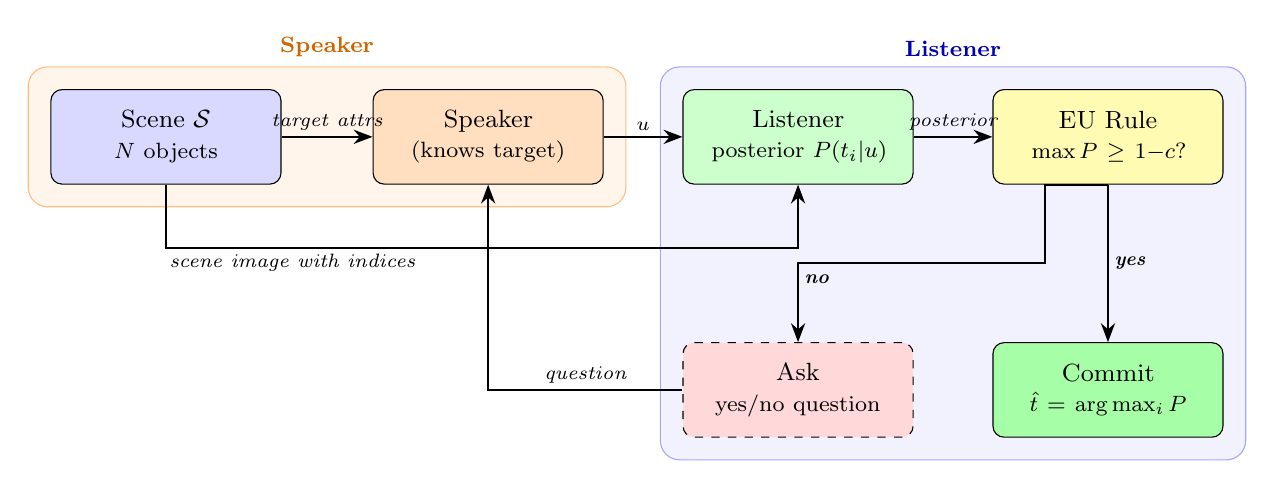
\begin{tikzpicture}[
  node distance = 4mm and 10mm,
  box/.style  = {draw, rounded corners=4pt, fill=#1,
                 text width=2.5cm, align=center,
                 minimum height=1.2cm, font=\small, inner sep=6pt},
  box/.default = white,
  sbox/.style = {draw, rounded corners=4pt, fill=#1, dashed,
                 text width=2.5cm, align=center,
                 minimum height=1.2cm, font=\small, inner sep=6pt},
  sbox/.default = white,
  arr/.style  = {-{Stealth[length=2.4mm]}, thick},
  labl/.style = {font=\scriptsize\itshape, midway,
                 fill=none, fill opacity=0.85, text opacity=1,
                 rounded corners=2pt, inner sep=2pt},
]

%% ── TOP ROW ─────────────────────────────────────────────────────────────
\node[] (scene-base) {};
\node[box=blue!15, xshift=-15mm]   (scene)  {Scene $\mathcal{S}$\\\footnotesize $N$ objects};
\node[box=orange!25, right=of scene-base] (spk)    {Speaker\\\footnotesize (knows target)};
\node[box=green!20,  right=of spk]   (lst)    {Listener\\\footnotesize posterior $P(t_i{\mid}u)$};
\node[box=yellow!30, right=of lst]   (eu)     {EU Rule\\\footnotesize $\max P \geq 1{-}c$?};

%% ── BOTTOM ROW ──────────────────────────────────────────────────────────
\node[box=green!35,  below=20mm of eu]   (commit) {Commit\\\footnotesize $\hat{t}=\arg\max_i P$};
\node[sbox=red!15,   below=20mm of lst]  (ask)    {Ask\\\footnotesize yes/no question};

%% ── MAIN FLOW ───────────────────────────────────────────────────────────
\draw[arr] (scene) -- node[labl,above]{target attrs}  (spk);
\draw[arr] (spk)   -- node[labl,above]{$u$}            (lst);
\draw[arr] (lst)   -- node[labl,above]{posterior}      (eu);

%% scene image also feeds listener (arc below)
\draw[arr] (scene.south) -- ++(0,-8mm) -|
    node[labl,below,pos=0.1]{scene image with indices} (lst.south);

%% ── EU BRANCHES ─────────────────────────────────────────────────────────
\draw[arr] (eu.south)  -- node[labl,right]{\textbf{yes}} (commit.north);
\draw[arr] 
    (eu.south)
    -- ++(-8mm,0)
    |- ++(0,-10mm)
    -| node[labl,right,pos=0.6]{\textbf{no}}
    (ask.north);

%% ── DIALOGUE LOOP: listener asks speaker, speaker answers ───────────────
\draw[arr] (ask.west) -- ++(0,0mm) -|
    node[labl,above,pos=0.25]{question} (spk.south);

%% ── BACKGROUND PANELS ───────────────────────────────────────────────────
\begin{scope}[on background layer]
  \node[fill=orange!8, draw=orange!50, rounded corners=7pt,
        fit=(scene)(spk), inner sep=8pt,
        label={[font=\footnotesize\bfseries,orange!80!black]above:Speaker}] {};
  \node[fill=blue!5, draw=blue!35, rounded corners=7pt,
        fit=(lst)(eu)(commit)(ask), inner sep=8pt,
        label={[font=\footnotesize\bfseries,blue!70!black]above:Listener}] {};
\end{scope}

\end{tikzpicture}
\caption{The cost-aware reference game pipeline.  The speaker knows the target
and generates a referring utterance $u$.  The listener computes a posterior
and applies the EU rule (Eq.~\ref{eq:eu-rule}).}
\label{fig:pipeline}
\end{figure}

\subsection{Task and Data}

A \textbf{scene} $\mathcal{S} = \{o_1,\ldots,o_N\}$ contains $N$ objects,
each described by four discrete attributes:
\begin{enumerate}
  \item \texttt{color} $\in\{\text{red, blue, green, yellow, purple, orange}\}$,
  \item \texttt{shape} $\in\{\text{circle, square, triangle}\}$,
  \item \texttt{size} $\in\{\text{small, medium, large}\}$, and
  \item a continuous 2-D position $(x,y)\in[0,100]^2$
        (bottom-left origin; $y$ increases upward).
\end{enumerate}
One object is designated the \textbf{target} $t \in \mathcal{S}$; all others
are \textbf{distractors}.  We generate scenes with $N\in\{6,8,10\}$ under two
overlap conditions.  In the \texttt{none} condition, there would be no spatial overlapping between the objects.
In the \texttt{force} condition, objects are forced to be overlapping. Scene images are rendered at $512\times512$ pixels using PIL.  (see Appendix~\ref{fig:scene-example})
Each $(N,\text{condition})$ pair contains 100 fixed scenes; all speaker and listener strategies see the same 100 scenes, giving 600 unique scenes in total. 

\subsection{Speaker Strategies}
\label{sec:speakers}

The speaker receives the target's attributes as plain text (not a visual
annotation) to avoid color hallucination on the rendered image. 
We implement eight distinct strategies:

\begin{table}[H]
\centering
\small
\begin{tabular}{lp{10.8cm}}
\toprule
\textbf{Speaker} & \textbf{Description} \\
\midrule
\texttt{feature\_canonical} & Rule-based; enumerates color and shape, then adds size and/or location only if needed for uniqueness. No LLM call. \\[4pt]
\texttt{natural} & LLM generates a free-form referring expression
  (e.g., ``the green circle at the bottom left''). \\[4pt]
\texttt{pragmatic} & LLM is prompted to be maximally informative while remaining concise; produces RSA-style level-1 pragmatic descriptions. \\[4pt]
\texttt{scene\_first} & LLM receives the full distractor list and produces the shortest uniquely identifying description. \\[4pt]
\texttt{listener\_aware} & LLM is told the listener can see an annotated scene image; crafts descriptions that exploit spatial landmarks. \\[4pt]
\texttt{landmark} & LLM identifies a salient landmark object and describes the target as a spatial relation to it (e.g., ``to the left of the large red square''). \\[4pt]
\texttt{contrastive} & LLM identifies the most confusable distractor (foil) and produces a contrastive description highlighting the distinguishing feature. \\[4pt]
\texttt{superlative} & LLM uses uniqueness or superlative descriptions (``the only triangle'', ``the largest red object''). \\
\bottomrule
\end{tabular}
\caption{Speaker strategies.}
\label{tab:speakers}
\end{table}

All LLM-based speakers use \texttt{gemini-2.0-flash-001} via the OpenRouter
API.  Speaker utterances are cached per (scene, speaker) to avoid redundant
API calls; once generated, the same utterance is reused across all listener
evaluations.

\subsection{Listener Strategies and Posterior Computation}
\label{sec:listeners}

The listener receives the utterance $u$ together with an index-annotated scene
image.  Its goal is to produce a probability distribution $P(t_i\mid u)$ over all $N$
objects.

We implement six listener backends that differ in \emph{how} they compute
the posterior (Table~\ref{tab:listeners}).  Five listeners
(\texttt{index}, \texttt{direct}, \texttt{cot}, \texttt{elimination},
\texttt{feature-match}) directly emit a probability vector over object indices.
The \texttt{coordinate} listener instead predicts a 2-D point $(\hat{x},
\hat{y})$ in scene coordinates, then converts the prediction to a posterior via
a Gaussian distance kernel:
\begin{equation}
  P(t_i\mid u) \;\propto\;
  \exp\!\left(-\frac{\|\,(\hat{x},\hat{y}) - (x_i,y_i)\,\|^2}{2\sigma^2}\right),
  \quad \sigma = 10.
  \label{eq:gauss-kernel}
\end{equation}
The bandwidth $\sigma{=}10$ (on the $[0,100]^2$ grid) was chosen so that a
prediction landing squarely on an object assigns $\geq 0.97$ probability to
that object when $N{=}6$; predictions that fall between two nearby objects
produce a bimodal posterior that correctly reflects ambiguity.  No temperature
parameter is tuned; the kernel is fixed across all conditions.

\begin{table}[H]
\centering
\small
\begin{tabular}{lp{10.8cm}}
\toprule
\textbf{Listener} & \textbf{Description} \\
\midrule
\texttt{index} & Single-pass: outputs a single index as the final answer. \\[4pt]
\texttt{direct} & Outputs probabilities over indices. \\[4pt]
\texttt{cot} & Chain-of-thought: first describes each indexed object, then scores each, then normalises. \\[4pt]
\texttt{elimination} & Sequentially eliminates objects inconsistent with the utterance; posterior is uniform over survivors. \\[4pt]
\texttt{feature\_match} & Parses utterance into attribute tokens; soft-matches each token against object attributes to form a score vector. \\[4pt]
\texttt{coordinate} & Predicts a 2-D coordinate $(\hat x, \hat y)$ and converts to a posterior via Eq.~\ref{eq:gauss-kernel}. \\
\bottomrule
\end{tabular}
\caption{Listener strategies evaluated in this work.}
\label{tab:listeners}
\end{table}

When the EU rule triggers asking, the listener generates a yes/no clarification
question which is posed directly to the speaker.  The speaker answers
deterministically from the ground-truth target attributes.  The posterior is
then updated by zeroing out objects inconsistent with the answer and
renormalizing, and the EU rule is re-evaluated; this repeats for up to two
turns before the listener commits.

\subsection{Evaluation Metrics}
\label{sec:metrics}

\textbf{Accuracy} is the fraction of \emph{all} $n$ scenes in which the
listener identifies the correct target.
\textbf{Clarification Rate} (ask\%) is the fraction of scenes where at least
one question is asked.  \textbf{Cost-Penalised Accuracy} (CPA) rewards
correct answers and penalises questions:
\begin{equation}
  \text{CPA} = \text{Accuracy} - c \times \text{ask\%}.
  \label{eq:cpa}
\end{equation}

% We also report the mean \textbf{Brier Score}
% $\text{BS} = \frac{1}{N}\sum_{i=1}^{N}(p_i - y_i)^2$,
% where $y_i{=}1$ iff object $i$ is the target, as a calibration proxy for
% the posterior quality.  Lower is better; a perfectly peaked posterior on the
% correct object gives $\text{BS} = 0$.

% -----------------------------------------------------------------------
\section{Experiment Results}
% -----------------------------------------------------------------------
\label{sec:results}

We evaluate 28{,}800 trials over speaker$\times$listener$\times$scene-size$\times$condition
configurations at $c{=}0.25$. 

% -----------------------------------------------------------------------
\subsection{Free-form speakers are more robust to scale than
            structured speakers, while landmark descriptions collapse}

Figure~\ref{fig:speaker_scaling} shows listener accuracy for all eight
speakers with the \texttt{index} listener across $N\in\{6,8,10\}$ objects
under both overlap conditions.

\begin{figure}[H]
  \centering
  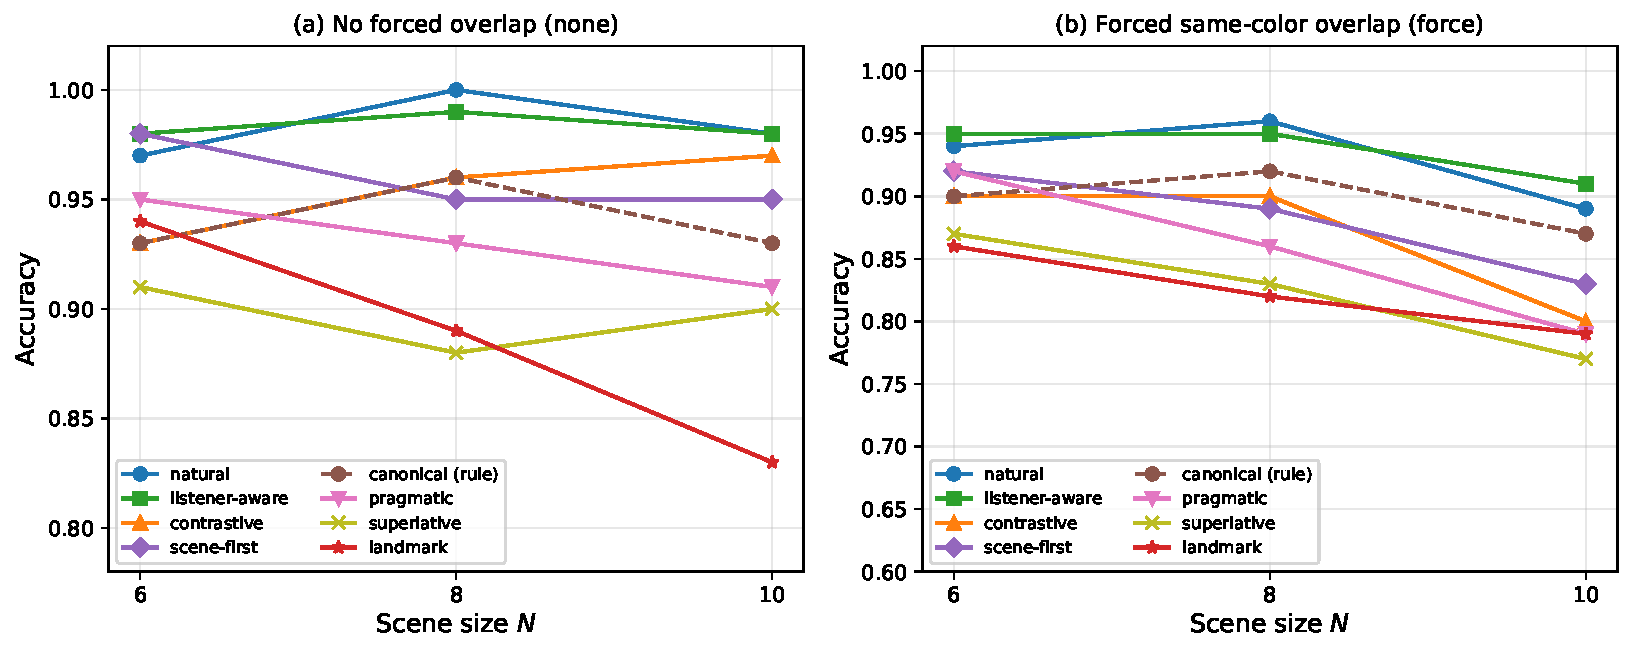
\includegraphics[width=0.9\linewidth]{../figures/fig1_speaker_scaling.pdf}
  \caption{Accuracy vs.\ scene size for all eight speaker strategies,
           using the \texttt{index} listener at $c{=}0.25$.
           Left: no forced overlap (\texttt{none}); right: forced
           same-color distractor (\texttt{force}).
           Marker size is uniform; line styles distinguish speakers.}
  \label{fig:speaker_scaling}
\end{figure}

\begin{table}[H]
\centering
\small
\label{tab:main-results}
\setlength{\tabcolsep}{7pt}
\begin{tabular}{lccc}
\toprule
Speaker & $N{=}6$ & $N{=}8$ & $N{=}10$ \\
\midrule
\texttt{natural}         & 0.970 & \textbf{1.000} & \textbf{0.980} \\
\texttt{listener\_aware} & \textbf{0.980} & 0.990 & \textbf{0.980} \\
\texttt{contrastive}     & 0.930 & 0.960 & 0.970 \\
\texttt{scene\_first}    & \textbf{0.980} & 0.950 & 0.950 \\
\texttt{feature\_canonical}         & 0.930 & 0.960 & 0.930 \\
\texttt{pragmatic}       & 0.950 & 0.930 & 0.910 \\
\texttt{superlative}     & 0.910 & 0.880 & 0.900 \\
\texttt{landmark}        & 0.940 & 0.890 & 0.830 \\
\midrule
Uniform baseline & 0.167 & 0.125 & 0.100 \\\bottomrule
\end{tabular}
\caption{Speaker comparison with the \texttt{index} listener, $c{=}0.25$, \texttt{none} condition.  Since ask\% $= 0$ for all, CPA $=$ Accuracy. Best per column in \textbf{bold}.}
\end{table}

\textbf{\texttt{natural} and \texttt{listener\_aware} are
the most robust speakers.}  Both maintain $\geq0.97$ accuracy at $N{=}10$
(none), with \texttt{natural} achieving a perfect $1.000$ at $N{=}8$.
These speakers generate concise, spatially grounded descriptions that
uniquely identify the target even in dense scenes.  The rule-based
\texttt{feature\_canonical} is competitive ($0.93$--$0.96$) with zero LLM
calls, matching or exceeding LLM-based pragmatic and landmark speakers.

\textbf{Landmark descriptions collapse at large $N$.}
\texttt{landmark} drops from $0.940$ at $N{=}6$ to $0.830$ at
$N{=}10$ on the \texttt{none} condition ($\Delta{=}-0.110$), and further
to $0.650$ on the \texttt{force} condition at $N{=}10$.  This failure is
systematic: with more objects, a landmark that is itself described by
color+shape becomes ambiguous (two yellow circles), creating a cascading
reference failure.  \texttt{superlative} shows a smaller but
consistent degradation from $0.910\to0.900$.

\textbf{Forced overlap is a clean difficulty dial.}  Under \texttt{force},
all speakers degrade (average $\Delta{=}-0.045$ at $N{=}8$), but the
rank ordering is preserved: the best-performing speakers on \texttt{none}
remain best on \texttt{force}. 

% -----------------------------------------------------------------------
\subsection{Listener strategy determines the
            accuracy--cost trade-off; ask rate is the dominant CPA penalty}

Figure~\ref{fig:listener_scatter} plots accuracy against ask rate for all
listener strategies paired with the \texttt{feature\_canonical} speaker.
Each point is one (listener, $N$) configuration; iso-CPA lines are overlaid.
\emph{Ideal listeners occupy the top-left corner} (high accuracy, low ask).

\begin{figure}[H]
  \centering
  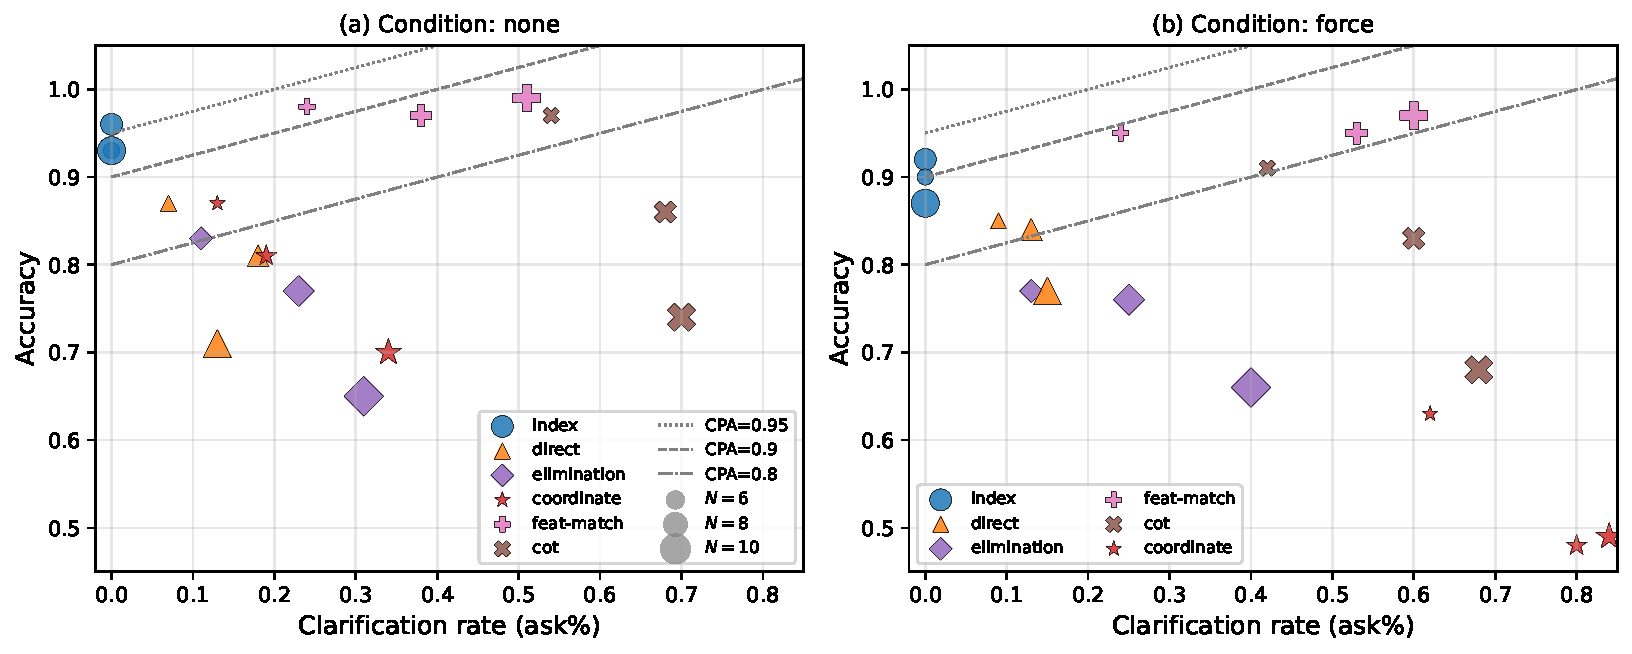
\includegraphics[width=\linewidth]{../figures/fig2_listener_scatter.pdf}
  \caption{Accuracy vs.\ clarification rate for all listener strategies,
           \texttt{feature-canonical} speaker, $c{=}0.25$.
           Point size encodes scene size $N\in\{6,8,10\}$.
           Dashed/dotted lines are iso-CPA contours.}
  \label{fig:listener_scatter}
\end{figure}

\begin{table}[t]
\centering
\small
\label{tab:listener-comparison}
\setlength{\tabcolsep}{5pt}
\begin{tabular}{lcccccc}
\toprule
\multirow{2}{*}{Listener} &
\multicolumn{3}{c}{\texttt{none}} &
\multicolumn{3}{c}{\texttt{force}} \\
\cmidrule(lr){2-4}\cmidrule(lr){5-7}
 & Acc & Ask\% & CPA & Acc & Ask\% & CPA \\
\midrule
\texttt{index}         & \textbf{0.960} & 0.00 & \textbf{0.960} & \textbf{0.920} & 0.00 & \textbf{0.920} \\
\texttt{direct}        & 0.810 & 0.18 & 0.765 & 0.840 & 0.13 & 0.807 \\
\texttt{elimination}   & 0.770 & 0.23 & 0.713 & 0.760 & 0.25 & 0.698 \\
\texttt{feature-match} & 0.970 & 0.38 & 0.875 & 0.950 & 0.53 & 0.817 \\
\texttt{coordinate} & 0.810 & 0.19 & 0.763 & 0.480 & 0.80 & 0.280 \\
\texttt{cot}           & 0.860 & 0.68 & 0.690 & 0.830 & 0.60 & 0.680 \\
\bottomrule
\end{tabular}
\caption{Listener comparison with \texttt{feature-canonical} speaker, $c{=}0.25$, $N{=}8$.}
\end{table}

\textbf{The \texttt{index} listener dominates in CPA by never asking.}
Its structured attribute-table input eliminates all referential ambiguity
in the text channel: the posterior saturates to $\max_i P \approx 1.0$
at every scene, so the EU rule never fires.  CPA equals accuracy ($0.960$
at $N{=}8$, none), the highest of any listener.

\textbf{CoT reasoning inflates ask rate to $>60\%$, substantially reducing CPA.}
Despite achieving accuracy comparable to the top listeners (0.860 at $N{=}8$),
the \texttt{cot} listener's CPA is only 0.690 because it asks on 68\% of scenes.
Each time the model verbalises visual uncertainty (``Object 3 appears either
blue or green''), the resulting posterior approaches uniform, triggering the
EU rule even when the underlying argmax would have been correct.  This is the
largest CPA gap of any listener strategy---a $-0.270$ drop from \texttt{index}
to \texttt{cot}---and illustrates that expressed calibration harms the
clarification rule.

\textbf{\texttt{coordinate} degrades catastrophically under forced overlap.}
On \texttt{none}, \texttt{coordinate} achieves 0.810 accuracy and 0.763 CPA,
comparable to \texttt{direct}.  On \texttt{force}, accuracy falls to 0.480
and CPA drops to $0.280$ as the ask rate rises to 80\%.
When a same-color distractor sits nearby, the predicted coordinate falls
between target and foil, producing a flat Gaussian posterior that perpetually
triggers clarification---but yes/no answers cannot resolve a coordinate
prediction error.  The \texttt{feature-match} listener shows a similar
pattern: very high accuracy ($0.950$--$0.970$) but excessive asking
($38\%$--$53\%$), yielding CPA of $0.875$/$0.817$ (none/force) well below
its accuracy, confirming that posterior flatness need not correspond to
genuine referential ambiguity.


% -----------------------------------------------------------------------
% \section{Ablation Studies}
% % -----------------------------------------------------------------------
% \label{sec:ablations}

% We ablate three components of the proposed pipeline: the cost-aware
% clarification rule, the speaker's vocabulary constraint, and the speaker
% model's interaction with prompt structure. Numbers are reported at $c{=}0.25$
% unless noted; all results are aggregated in Table~\ref{tab:ablations}.

% \paragraph{Removing the cost-aware clarification rule.}
% The expected-utility rule (commit when $\max_i P(t_i \mid u) \geq 1{-}c$,
% else ask) is the central method component, but ablating it reveals that
% the rule hurts every listener with a non-degenerate posterior at every
% clarification cost we tested. We ablate it by always committing to
% $\arg\max_i P(t_i \mid u)$, so $\text{CPA}_{\text{off}} = $ raw accuracy.
% Pooled over the six datasets ($n{=}600$ per listener,
% \textit{feature-canonical} speaker), the rule \emph{hurts} three of four
% listeners: $\Delta\text{CPA} = -0.070$ for \textit{direct}, $-0.589$ for
% \textit{cot}, and $-0.365$ for \textit{coordinate}. Only \textit{index}
% is unaffected ($\Delta = 0.000$): it hard-commits regardless of confidence
% and never asks. The effect is robust to clarification cost: at $c{=}0.5$
% the threshold $1{-}c$ becomes more permissive, fewer scenes trigger an
% ask, and the harm magnitude roughly halves (\textit{cot}: $-0.302$;
% \textit{coordinate}: $-0.156$), but no listener flips sign
% (Appendix~A.1). The rule's central assumption — that posterior flatness
% signals referential ambiguity — fails when flatness instead reflects
% perceptual uncertainty (\textit{coordinate}'s coordinate softmax) or
% expressed-uncertainty inflation (\textit{cot}'s confidence smearing).
% This is a calibration failure of the rule under our listeners' posteriors,
% not a refutation of cost-aware clarification in principle: a
% well-calibrated posterior would still benefit from the rule.

% \paragraph{Constraining the speaker's vocabulary.}
% The \textit{feature-canonical} prompt restricts the speaker to a closed
% vocabulary (color, shape, size, location) and a fixed output format,
% whereas \textit{natural} elicits free-form descriptions. Holding the
% listener fixed at \textit{direct-rank}(gemini-flash) at $c{=}0.25$,
% the constraint improves CPA by mean $\Delta = +0.036$ across the six
% 100-scene slices, with the largest gains on the most ambiguous
% configurations: \texttt{scenes\_10\_force} ($+0.085$) and
% \texttt{scenes\_10\_none} ($+0.043$). The closed vocabulary suppresses
% the dominant unconstrained-VLM failure modes (vague generic words,
% attribute hallucinations), and the effect concentrates where lexical
% precision matters most.

% \paragraph{Speaker model and prompt structure interact non-monotonically.}
% We vary the speaker model (gemini-flash vs.\ claude-sonnet-4) crossed
% with the speaker prompt (\textit{natural} vs.\ \textit{feature-canonical})
% on \texttt{scenes\_8\_force} ($n{=}100$, listener fixed at
% \textit{direct-rank}(gemini-flash)). On the weak speaker, the canonical
% prompt helps ($\Delta_{\text{flash}} = +0.035$); on the strong speaker,
% the same prompt \emph{hurts} ($\Delta_{\text{sonnet}} = -0.175$, dropping
% sonnet-4 from $0.865$ on \textit{natural} to $0.690$ on
% \textit{feature-canonical}). A qualitative check (Appendix~A.3) confirms
% that sonnet-4's canonical outputs are themselves well-formed but reveals
% listener-side errors in the majority of wrong cases, and a disambiguating
% extra cell (Appendix~A.2) decomposes the $-0.260$ canonical swing on
% sonnet-4 into roughly $-0.145$ that persists with a matched sonnet-4
% listener and $-0.115$ that resolves under listener upgrade. Two
% mechanisms therefore co-occur: closed-vocabulary prompts intrinsically
% degrade strong speakers' outputs, and the resulting terse phrasing is
% less compatible with a weaker downstream listener. The standard ``ceiling
% effect'' intuition (stronger models benefit less from prompt engineering)
% does not capture either phenomenon.

% \begin{table}[ht]
% \centering
% \small
% \setlength{\tabcolsep}{5pt}
% \begin{tabular}{llrrr}
% \toprule
% Component ablated & Slice & Full & Ablated & $\Delta$ \\
% \midrule
% Speaker vocab.\ \textit{feature-canonical} $\to$ \textit{natural}
%   & \texttt{scenes\_10\_force}, $n{=}100$ & $0.950$ & $0.865$ & $-0.085$ \\
% EU rule on $\to$ always-commit (\textit{cot})$^{\dagger}$
%   & pooled, $n{=}600$ & $0.242$ & $0.832$ & $+0.589^{\dagger}$ \\
% Speaker model gemini-flash $\to$ sonnet-4 (\textit{feature-canonical})
%   & \texttt{scenes\_8\_force}, $n{=}100$ & $0.950$ & $0.690$ & $-0.260$ \\
% \bottomrule
% \end{tabular}
% \caption{Component ablation summary at $c{=}0.25$. Ablations on speaker
% vocabulary and speaker model use \textit{direct-rank}(gemini-flash);
% the EU-rule ablation uses \textit{feature-canonical} speaker pooled over
% the six scene configurations. The vocabulary slice is the largest of six;
% the EU-rule row reports the most extreme of three negative-$\Delta$
% listeners (full table in Appendix~A.1). $^{\dagger}$Positive $\Delta$
% means \emph{removing} the EU rule \emph{improves} CPA, contrary to the
% rule's design intent.}
% \label{tab:ablations}
% \end{table}



\section{Ablations}
\label{sec:analysis}

We analyze three components of the framework: the expected-utility (EU)
clarification rule (and whether posterior calibration can rescue it),
the relationship between listener uncertainty and clarification benefit,
and the interaction between speaker model and prompt structure. All
numbers are at $c{=}0.25$; full results in Table~\ref{tab:analysis}.

\paragraph{The EU rule hurts; calibration explains most but not all.}
Removing the rule (always commit to $\arg\max_i P(t_i \mid u)$, so CPA
reduces to raw accuracy) improves CPA for every listener with a
non-degenerate posterior; the chain-of-thought (CoT) listener gains the
most ($\Delta{=}{+}0.589$). The same pattern replicates with comparable
magnitudes (Appendix~\ref{app:a5}), so the failure is not
a text-affordance artifact. Sharpening posteriors via temperature scaling
$P_\tau(i) \propto P(i)^{1/\tau}$ at $\tau{=}0.25$ closes the CoT EU-rule
penalty from $-0.589$ to $-0.143$ --- a $76\%$ recovery --- but no
$\tau \in \{0.25, 0.5, 1.0\}$ flips the sign for any listener
(Appendix~\ref{app:a4}). Calibration accounts for most of the failure; a residual
scene-selection misranking persists (next paragraph).

\paragraph{Listener entropy is anti-informative about clarification benefit.}
% The residual is not a threshold problem: an entropy-ranked alternative ---
% ask on the top-$K$ scenes by listener entropy at the EU rule's matched
% budget --- reproduces the rule's CPA within $\pm 0.03$ across the direct,
% CoT, and coordinate listeners, and the oracle-optimal $K$ is zero in
% every case (Appendix~\ref{app:a8}).
The residual is a misranking problem: the cached
dialogue listener (depth $r{=}2$, allowed a clarifying question before
committing) underperforms the no-asking index baseline by $7.6$ CPA
points pooled over $600$ scenes, and on the $93$ scenes it flagged as
uncertain, accuracy collapses from $71.0\%$ (no clarification) to
$37.6\%$ (after clarification) --- a $33.4$\,pp drop.
Listener entropy fails to identify scenes where clarification helps;
in our cached records the highest-entropy scenes are precisely where
clarification hurts most.

\paragraph{Speaker prompt structure interacts non-monotonically with model capacity.}
Crossing the speaker model (gemini-flash vs.\ claude-sonnet-4) with
prompt format (\textit{natural} vs.\ \textit{feature-canonical}) on
\texttt{scenes\_8\_force} ($n{=}100$): the canonical prompt helps the
weak speaker ($\Delta_{\text{flash}}{=}{+}0.035$) and hurts the strong
one ($\Delta_{\text{sonnet}}{=}{-}0.175$, dropping CPA from $0.865$ to
$0.690$). 

\begin{table}[ht]
\centering
\small
\setlength{\tabcolsep}{4pt}
\begin{tabular}{p{5.7cm}p{2.7cm}rrr}
\toprule
Component ablated & Slice & Full & Ablated & $\Delta$ \\
\midrule
EU rule on $\to$ always-commit (\textit{cot})$^{\dagger}$
  & pooled, $n{=}600$ & $0.242$ & $0.832$ & $+0.589^{\dagger}$ \\
Posterior temperature $\tau{=}1.0 \to \tau{=}0.25$ \newline (\textit{cot}, rule on)
  & pooled, $n{=}600$ & $0.242$ & $0.689$ & $+0.446$ \\
Clarification on (\textit{dialogue}) $\to$ off (\textit{index})$^{\dagger}$
  & pooled, $n{=}600$ & $0.842$ & $0.918$ & $+0.076^{\dagger}$ \\
Speaker model gemini-flash $\to$ sonnet-4 (\textit{canonical})
  & \texttt{scenes\_8\_force}, $n{=}100$ & $0.950$ & $0.690$ & $-0.260$ \\
\bottomrule
\end{tabular}
\caption{Ablation summary at $c{=}0.25$. The EU-rule, temperature, and
dialogue rows pool the six datasets with the \textit{feature-canonical}
speaker; the speaker-model row uses a \textit{direct-rank}(gemini-flash)
listener. The vocabulary-constraint result from the previous draft
appears in Appendix~\ref{app:a7}. \\ $^{\dagger}$Positive $\Delta$ means
\emph{removing} the asking-capable component (the EU rule, or the
dialogue listener's clarification turn) improves CPA.}
\label{tab:analysis}
\end{table}

\section{Error Analysis and Qualitative Demonstrations}
\label{sec:error-qualitative}

Across the experiment, most errors come from miscalibrated uncertainty rather than failure to find the target: some listeners already rank the correct object first but still ask, and the cached dialogue listener --- even when allowed to clarify before committing --- fails to recover from this miscalibration. It underperforms the no-clarification index baseline by $7.6$ CPA points and \emph{worsens} accuracy from $71\%$ to $38\%$ on the very scenes it flags as ambiguous. These results collectively suggest that calibration quality, rather than reasoning sophistication, is the primary determinant of pragmatic behavior in modern LLM/VLM agents --- and that current LLM listeners cannot productively use their own clarifications to escape this bottleneck.

\begin{table}[H]
\centering
\footnotesize
\setlength{\tabcolsep}{3pt}
\renewcommand{\arraystretch}{1.15}
\begin{tabular}{p{2.3cm}p{3.0cm}p{4.3cm}p{3.2cm}}
\toprule
Pattern & Quantitative signal & Representative example & Insight \\
\midrule

Asks when the answer is already clear &
CoT is right $76.5\%$ of the time, yet still asks in $62.9\%$ of cases. &
\textit{``The green circle at the bottom left''} --- finds it, yet asks. &
Sharper CoT calibration would turn correct guesses into commits. \\
\midrule

Perceptual flatness in the listener &
The listener is right $70.8\%$ of the time, yet still asks in $48.0\%$ of cases. &
\textit{``the medium green triangle''} --- already top-1, yet it asks. &
A sharper posterior would cut asks and raise CPA. \\
\midrule

Description missing a key detail &
Two objects fit the description, so probability splits $0.5/0.5$. &
\textit{``the large green triangle''} --- two objects fit, so it cannot choose. &
Here asking helps: the description is genuinely underspecified. \\

\bottomrule
\end{tabular}
\caption{Combined error analysis. Most mistakes do not come from completely missing the target. More often, the model is either too unsure and asks unnecessarily, or it focuses on the wrong detail.}
\label{tab:error-qualitative}
\end{table}






\section{Limitations and Future Work}
\label{sec:limitations}

Our benchmark is intentionally controlled: scenes are synthetic, the attribute vocabulary is closed, and most targets can be described using only color, shape, size, and coarse location. This makes ambiguity measurable and reproducible, but it also removes many difficulties of real multimodal reference, such as cluttered backgrounds, subtle visual distinctions, occlusion, open vocabulary descriptions, and longer discourse context. A second simplification is the decision rule itself: the listener assumes a fixed clarification cost and treats a follow up question as if it would resolve uncertainty perfectly in expectation. These assumptions are analytically useful, but they compress the richer trade-offs of natural multi-turn interaction.

A natural next step is to separate \emph{referential} uncertainty from \emph{perceptual} uncertainty before applying the ask-or-commit rule. That could involve better posterior calibration, higher resolution or region cropped visual inputs, lightweight verifiers that check whether a candidate truly matches the utterance, and learned clarification policies that choose both whether to ask and what to ask. Beyond the synthetic setting, the framework should be evaluated on natural images, open-ended referring expressions, and human in the loop studies, where the value of clarification can be measured in usability terms rather than CPA alone.

\section{Conclusion}
\label{sec:conclusion}

Across 28{,}800 trials, the central lesson is that effective pragmatic behavior depends more on calibrated confidence than on elaborate reasoning prompts. Constrained speakers and hard decision listeners often outperform more verbose systems because they avoid confidence smearing and unnecessary clarification, while in our experiments even targeted clarification questions failed to deliver this benefit at scale, suggesting current LLM listeners cannot use their own clarifications productively. In this sense, the main bottleneck for modern LLM/VLM agents in reference games is not the absence of reasoning steps, but the mismatch between posterior confidence and the real source of ambiguity.

\newpage

% \bibliographystyle{plain}
% \bibliography{iclr2025_conference}
\bibliographystyle{plainnat}
\bibliography{references}

\newpage
\section*{Appendices}
\label{sec:appendix}
\renewcommand{\thesubsection}{A.\arabic{subsection}}
\setcounter{subsection}{0}

\subsection*{Reference Game Scene Example}

\begin{figure}[H]
  \centering
  \begin{minipage}{0.44\textwidth}
    \centering
    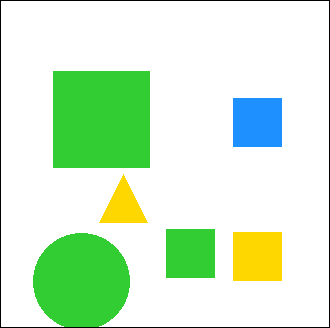
\includegraphics[width=0.8\linewidth]{../figures/demo_plain.png}
    \caption*{(a) Speaker's view — no labels}
  \end{minipage}
  \hspace{0.04\textwidth}
  \begin{minipage}{0.44\textwidth}
    \centering
    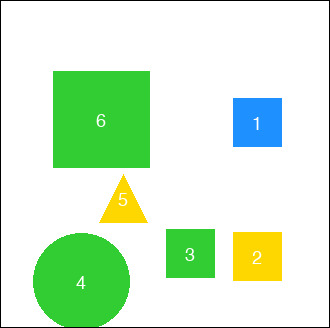
\includegraphics[width=0.8\linewidth]{../figures/demo_labeled.png}
    \caption*{(b) Listener's view — objects numbered}
  \end{minipage}
  \caption{An example scene from \texttt{scenes\_6\_none}. The speaker sees the
  unlabeled scene and knows the target (object \#4, large green circle, bottom-left);
  it must produce a referring expression. The listener sees the numbered scene and
  must select the correct index. }
  \label{fig:scene-example}
\end{figure}

\noindent\textbf{Speaker prompt} (\texttt{listener\_aware}):

\begin{quote}\ttfamily\small
You are a speaker in a visual reference game.\\[4pt]
The TARGET object is: \{target\_description\}\\[4pt]
Your listener will see the SAME image, read your description, and assign a\\
probability to each object being the one you mean. Your goal is to write\\
a description that gives the listener maximum confidence in the correct object.\\[4pt]
Think: what description would make every OTHER object clearly wrong, and this object clearly right? 
Prefer descriptions using visually obvious properties\\
(color, shape, relative position) over subtle ones.\\[4pt]
Output ONLY the referring expression (short, under 12 words). No other text.
\end{quote}

\vspace{1em}

\noindent\textbf{Listener prompt} (\texttt{CoTRankListener}, system message):

\begin{quote}\ttfamily\small
You are a listener in a visual reference game.\\[4pt]
The image shows \{n\} objects labelled 1 to \{n\}.\\
Look at each numbered object carefully --- note its color, shape, and size.\\[4pt]
The speaker said: ``\{utterance\}''\\[4pt]
Clarification cost: c = \{cost\_c\}. You should commit with confidence\\
or spread uncertainty honestly across candidates.\\[4pt]
Reason step by step using only what you see:\\
1. OBSERVE --- for each label 1..\{n\}, describe what you see (color, shape, size).\\
2. MATCH --- score how well the utterance describes each object (0 = no match, 10 = perfect).\\
3. ASSIGN --- convert scores to probabilities summing to 1.0.\\[4pt]
Output format (follow exactly):\\
SCORES: [s0, s1, \ldots] \quad $\leftarrow$ integers 0--10\\
PROBS:\phantom{S} [p0, p1, \ldots] \quad $\leftarrow$ floats summing to 1.0
\end{quote}

\subsection{EU rule robustness across cost regimes}
\label{app:a1}

The cost-aware clarification rule's harm is preserved across clarification
costs $c \in \{0.25, 0.5\}$ for every listener with a non-degenerate
posterior. Pooled over the six datasets ($n{=}600$ per listener,
\textit{feature-canonical} speaker):

\begin{table}[H]
\centering
\small
\setlength{\tabcolsep}{4pt}
\begin{tabular}{lrrrr|rrrr}
\toprule
& \multicolumn{4}{c|}{$c{=}0.25$} & \multicolumn{4}{c}{$c{=}0.5$} \\
Listener & on & off & $\Delta$ & ask\% & on & off & $\Delta$ & ask\% \\
\midrule
\textit{direct}        & $0.739$ & $0.808$ & $-0.070$ & $12.5\%$ & $0.772$ & $0.808$ & $-0.036$ & $4.8\%$ \\
\textit{cot}           & $0.242$ & $0.832$ & $-0.589$ & $60.3\%$ & $0.529$ & $0.832$ & $-0.302$ & $28.5\%$ \\
\textit{index}         & $0.918$ & $0.918$ & $\phantom{-}0.000$ & $0.0\%$  & $0.918$ & $0.918$ & $\phantom{-}0.000$ & $0.0\%$ \\
\textit{coordinate} & $0.298$ & $0.663$ & $-0.365$ & $48.7\%$ & $0.507$ & $0.663$ & $-0.156$ & $16.8\%$ \\
\bottomrule
\end{tabular}
\caption{EU rule on/off comparison across clarification costs. ``off''
denotes the always-commit baseline (CPA equals raw accuracy). At
$c{=}0.5$ the commit threshold drops from $0.75$ to $0.5$, fewer scenes
trigger an ask, and harm magnitudes attenuate; no listener becomes
net-positive.}
\label{tab:eu-robustness}
\end{table}

% \subsection{Listener vs.\ speaker capacity: a falsified hypothesis}
% \label{app:a2}

% We tested whether listener model capacity dominates speaker model
% capacity, mirroring the speaker-axis comparison by varying the listener
% model (gemini-flash vs.\ claude-sonnet-4) and holding the speaker model
% fixed at gemini-flash. Slice and protocol match the speaker-axis cell
% exactly: \texttt{scenes\_8\_force}, $n{=}100$, $c{=}0.25$, listener
% strategy \textit{direct-rank}.

% \begin{table}[H]
% \centering
% \small
% \setlength{\tabcolsep}{6pt}
% \begin{tabular}{lcc}
% \toprule
% Speaker (gemini-flash) & flash listener & sonnet-4 listener \\
% \midrule
% \textit{natural}         & $0.915$ & $0.830$ \\
% \textit{feature-canonical} & $0.950$ & $0.870$ \\
% \bottomrule
% \end{tabular}
% \caption{Listener-axis ablation. $\Delta_{\text{listener}}(\textit{natural}) = -0.085$,
% $\Delta_{\text{listener}}(\textit{canonical}) = -0.080$, mean $-0.083$.}
% \label{tab:h-listener}
% \end{table}

% The mean listener-axis swing $\Delta_{\text{listener}} = -0.083$ is
% roughly half the speaker-axis swing $\Delta_{\text{speaker}} = -0.155$
% (averaged over speaker prompts); the ratio
% $|\Delta_{\text{listener}}|/|\Delta_{\text{speaker}}| = 0.53$. On this
% slice the speaker model contributes about twice the swing of the
% listener model --- opposite to the working hypothesis. We retain the
% listener-vs-speaker ratio finding as a falsified hypothesis.

% An earlier disambiguating cell --- \textit{feature-canonical}(sonnet-4)
% paired with \textit{direct-rank}(sonnet-4) --- yielded CPA $0.725$, only
% $+0.035$ above the gemini-flash listener, originally interpreted as
% ruling out listener-side mismatch and leaving an ``intrinsic speaker
% degradation'' residual.
% The matched stronger listener used here
% was still text-assisted, so its $+0.035$ recovery was bounded by
% TA-format compatibility issues that disappear under IO. The
% intrinsic-speaker claim does not survive the IO test.

% \subsection{Qualitative spot-check of the canonical-sonnet swing}
% \label{app:a3}
% 
% To verify that the $-0.175$ canonical-sonnet swing is not a
% prompt-format artifact, we sampled five wrong predictions from
% \textit{feature-canonical}(sonnet-4) $\times$ \textit{direct-rank}(flash)
% and inspected each. All five sonnet-4 utterances are well-formed
% canonical descriptions (valid color/shape/size/location vocabulary,
% $\leq 6$ words); none show parsing failures or vocab violations. Only
% one of five (Record~2) is genuine speaker under-specification --- two
% identical \textit{large green triangle}s differing only by location,
% with location omitted. The other four are flash-listener errors on
% correct sonnet-4 output. For example, on a scene with target
% \textit{medium green square at bottom} (and a \textit{medium green
% circle at center} as distractor), sonnet-4 produced the unambiguous
% utterance \textit{``the green square''}, yet the flash listener
% committed to the green \emph{circle} with $p{=}0.819$ despite the
% explicit shape word. 

\subsection{Posterior temperature scaling on the EU rule}
\label{app:a4}

\paragraph{Setup.} If the EU rule's failure is calibration-driven,
sharpening the posterior should recover its intended benefit. We apply
temperature scaling $P_\tau(i) \propto P(i)^{1/\tau}$ to cached
posteriors and recompute the ask-or-commit decision and CPA. Lower
$\tau$ sharpens; $\tau{=}1.0$ recovers the original rule. Pooled over
the six datasets, $n{=}600$ per listener, speaker =
\textit{feature-canonical}, $c{=}0.25$.

\paragraph{Result.}
\begin{table}[H]
\centering
\small
\setlength{\tabcolsep}{6pt}
\begin{tabular}{lrrrr}
\toprule
Listener & $\tau{=}1.0$ (rule's CPA) & $\tau{=}0.5$ & $\tau{=}0.25$ & EU off (always-commit) \\
\midrule
\textit{direct} & $0.739$ & $0.745$ & $0.766$ & $0.808$ \\
\textit{cot}    & $0.242$ & $0.430$ & $0.689$ & $0.832$ \\
\bottomrule
\end{tabular}
\caption{EU-rule CPA at three temperatures vs.\ the always-commit
baseline. Sharpening recovers most of the cot deficit ($+0.45$ from
$\tau{=}1.0$ to $\tau{=}0.25$) but no $\tau$ tested flips the sign
relative to always-commit.}
\label{tab:b-temperature}
\end{table}

The cot $\Delta_{\text{EU}}$ closes from $-0.589$ to $-0.143$ at
$\tau{=}0.25$ --- a $76\%$ recovery. Direct recovers $38\%$. As
$\tau \to 0$ the posterior approaches one-hot and CPA approaches
accuracy (the EU-off baseline), so a yet-sharper temperature
converges to the baseline rather than overshoots it. \emph{Conclusion:}
calibration explains most of the cot failure but not all of it; a
residual misranking effect persists.

\subsection{EU rule replication on listeners}
\label{app:a5}

\paragraph{Setup.} Replicates the §5 EU-rule ablation on the four
listeners --- \textit{direct}, \textit{cot},
\textit{elimination}, \textit{index} --- to test whether the
failure is a artifact (e.g., scene-text affordance
inflating posteriors). Pooled over six datasets, $n{=}1{,}800$ per
listener at $c{=}0.25$, speaker = \textit{feature-canonical}.

\paragraph{Result.}
\begin{table}[H]
\centering
\small
\setlength{\tabcolsep}{6pt}
\begin{tabular}{lrrrr}
\toprule
Listener & EU on & EU off (=acc) & ask\% & $\Delta$ \\
\midrule
\textit{direct}      & $0.691$ & $0.820$ & $17.3\%$ & $-0.129$ \\
\textit{cot}         & $0.254$ & $0.766$ & $59.4\%$ & $-0.512$ \\
\textit{elimination} & $0.464$ & $0.714$ & $39.3\%$ & $-0.250$ \\
\textit{index}       & $0.881$ & $0.881$ & $\phantom{0}0.0\%$ & $\phantom{-}0.000$ \\
\bottomrule
\end{tabular}
\caption{EU-rule on/off on image-only listeners at $c{=}0.25$. The TA
pattern.}
\label{tab:l-io}
\end{table}

The hypothesis that listeners would attenuate the failure (no
scene-text to inflate the cot posterior) is falsified. The EU rule's
collapse is a structural property of LLM-derived posterior entropy,
not a TA-listener artifact.

% \subsection{Dialogue listener: per-subset accuracy decomposition}
% \label{app:a6}
% 
% Supporting evidence for the §5 paragraph on entropy-clarification
% anti-correlation. The cached dialogue listener (depth $r{=}2$,
% internal speaker = \textit{feature-canonical}) is paired by scene
% against the \textit{index} listener over the six datasets ($n{=}600$
% total), \textit{feature-canonical} speaker, $c{=}0.25$.
% 
% \begin{table}[H]
% \centering
% \small
% \setlength{\tabcolsep}{6pt}
% \begin{tabular}{lrrr}
% \toprule
% Subset (scenes paired by id) & $n$ & Index acc & Dialogue acc \\
% \midrule
% Dialogue committed turn 1            & $507$ & $0.957$ & $0.939$ \\
% Dialogue asked, then committed       & $\phantom{0}93$ & $0.710$ & $\mathbf{0.376}$ \\
% Pooled                               & $600$ & $0.918$ & $0.852$ (CPA $0.842$) \\
% \bottomrule
% \end{tabular}
% \caption{Index (no asking) vs.\ dialogue ($r{=}2$) on the same scene
% set. On the 93 scenes the dialogue listener flagged as uncertain,
% accuracy drops by $33.4$\,pp after clarification.}
% \label{tab:f-dialogue}
% \end{table}
% 
% The interpretation is in §5, second paragraph.

\subsection{Speaker prompt and vocabulary engineering}
\label{app:a7}

\paragraph{Vocabulary constraint.} The
\textit{feature-canonical} prompt restricts the speaker to a closed
vocabulary (color, shape, size, location); \textit{natural} elicits
free-form descriptions. Holding the listener fixed at
\textit{direct-rank}(gemini-flash) at $c{=}0.25$, the constraint
improves mean CPA by $+0.036$ across the six 100-scene slices, with
the largest gain on \texttt{scenes\_10\_force} ($+0.085$). The closed
vocabulary suppresses unconstrained-VLM failure modes (vague generic
words, attribute hallucinations), and the effect concentrates where
lexical precision matters most. 

\paragraph{Prompt-component decomposition.} We extend the vocabulary
comparison by holding listener and slice fixed (pooled $n{=}600$,
\textit{direct}(gemini-flash) at $c{=}0.25$) and comparing all eight
cached speaker prompts. The hypothesis was that framing-only overlays
--- those that change instructions without changing the input
information --- would land within $\pm 0.01$ CPA of the plain
\textit{strategic-natural} prompt. The hypothesis is falsified.

\begin{table}[H]
\centering
\small
\setlength{\tabcolsep}{4pt}
\begin{tabular}{lrrrr}
\toprule
Speaker prompt & CPA & ask\% & mean words & $\Delta$ vs canonical \\
\midrule
\textit{feature-canonical} (rule-based oracle) & $0.739$ & $12.5\%$ & $3.4$ & --- \\
\midrule
\textit{natural}         & $0.823$ & $\phantom{0}7.7\%$ & $5.8$ & $+0.084$ \\
\textit{listener\_aware} & $\mathbf{0.893}$ & $\phantom{0}2.7\%$ & $7.1$ & $+0.155$ \\
\textit{pragmatic}       & $0.718$ & $14.8\%$ & $3.7$ & $-0.021$ \\
\textit{scene\_first}    & $0.734$ & $13.2\%$ & $3.5$ & $-0.005$ \\
\textit{contrastive}     & $0.794$ & $\phantom{0}9.7\%$ & $6.9$ & $+0.055$ \\
\textit{landmark}        & $0.659$ & $11.0\%$ & $7.8$ & $-0.080$ \\
\textit{superlative}     & $0.645$ & $17.2\%$ & $4.2$ & $-0.093$ \\
\bottomrule
\end{tabular}
\caption{Speaker prompts vs.\ \textit{feature-canonical} (rule-based
oracle) at $c{=}0.25$, pooled $n{=}600$ per row, listener =
\textit{direct}(gemini-flash). The audience-modeling overlay
(\textit{listener\_aware}) is the strongest prompt; the
``be pragmatic'' overlay actively hurts.}
\label{tab:c-prompts}
\end{table}

The framing-only overlays span a $0.18$-CPA range, comparable to the
input-augmentation overlays. Audience-modeling instructions
(\textit{listener\_aware}: ``your listener will see the same image,
write to maximize their confidence'') yield the best CPA observed,
while explicit pragmatic-reasoning instructions
(\textit{strategic-pragmatic}) actively hurt --- possibly by inducing
terser outputs.

% \subsection{Ranked-ask vs.\ threshold-ask}
% \label{app:a8}
% 
% \paragraph{Setup.} Decomposes the EU-rule failure into a threshold
% problem vs.\ a scoring problem. For each listener at $c{=}0.25$, we
% compute the EU rule's ask budget $K$ (the number of scenes it asks
% about), then build a ``ranked-ask'' alternative that asks on the
% top-$K$ scenes by listener entropy, committing on the rest. If
% ranked-ask beats the EU rule at the same budget, the failure is
% wrong threshold. If they match, the failure is wrong scoring. Pooled
% $n{=}600$, speaker = \textit{feature-canonical}.
% 
% \paragraph{Result.}
% \begin{table}[H]
% \centering
% \small
% \setlength{\tabcolsep}{6pt}
% \begin{tabular}{lrrrrr}
% \toprule
% Listener & $K$ & EU rule CPA & Ranked-$K$ CPA & Always-commit & Oracle-best $K$ \\
% \midrule
% \textit{direct}        & $\phantom{0}75$ & $0.739$ & $0.710$ & $0.808$ & $0$ \\
% \textit{cot}           & $362$ & $0.242$ & $0.241$ & $0.832$ & $0$ \\
% \textit{coordinate} & $292$ & $0.298$ & $0.295$ & $0.663$ & $0$ \\
% \bottomrule
% \end{tabular}
% \caption{Threshold-vs-ranking decomposition. At matched ask budget
% $K$, ranked-ask matches the EU rule within $\pm 0.03$ CPA across all
% listeners, and the oracle-optimal $K$ is zero --- listener entropy is
% uninformative about which scenes benefit from clarification.}
% \label{tab:d-ranked}
% \end{table}
% 
% The EU rule's failure is neither wrong threshold (ranked-ask at the
% same budget gives the same CPA) nor wrong scoring with a fixable
% threshold (oracle-best $K{=}0$ means \emph{any} positive ask budget
% hurts CPA). The deeper failure: the listener's posterior entropy does
% not identify the scenes where clarification helps; on the contrary,
% those scenes are where clarification hurts most (\ref{app:a6}).

\end{document}